\documentclass[twocolumn]{aastex631}

\usepackage{amsmath}
\usepackage{multirow}
\usepackage{natbib}
\usepackage{graphicx} 
\usepackage{aas_macros}

\begin{document}

\subsection{Data Preprocessing and Dataset Characteristics}

The initial dataset consisted of 1000 merger trees extracted from cosmological N-body simulations. Each node in these trees represents a dark matter halo, characterized by four features: halo mass, halo concentration, maximum circular velocity ($V_{max}$), and scale factor (ranging from 0 to 1). The edges represent merger events.

\subsubsection{Feature engineering and normalization}
As described in the methods section, node features underwent a preprocessing step to improve the distribution of the data. Halo mass and $V_{max}$ were log$_{10}$-transformed to reduce skewness, given their large dynamic ranges. All four node features (log$_{10}$(Mass), Concentration, log$_{10}$($V_{max}$), Scale Factor) were then normalized to a range between 0 and 1 across the dataset. The normalization parameters, derived from the subset of data for which the assembly bias proxy could be computed, were:
\begin{itemize}
    \item Log$_{10}$(Mass): Min = 0.983, Max = 1.167
    \item Concentration: Min = 0.0002, Max = 3.767
    \item Log$_{10}$($V_{max}$): Min = 0.194, Max = 0.499
    \item Scale Factor: Min = 0.077, Max = 1.0
\end{itemize}

Edge features were engineered to capture information about the merger events. These included:
\begin{enumerate}
    \item Mass Ratio: The ratio of the smaller halo mass to the larger halo mass involved in a merger.
    \item Time Difference: The absolute difference in scale factors between the merging halos.
\end{enumerate}
These engineered edge features were also normalized to a range between 0 and 1:
\begin{itemize}
    \item Mass Ratio: Min = 0.714, Max = 1.0
    \item Time Difference: Min = 0.003, Max = 0.776
\end{itemize}

\subsubsection{Assembly bias proxy calculation and dataset reduction}
A critical step was the calculation of an assembly bias proxy for each merger tree. As described in the methods section, this proxy was defined as the mean halo mass of the main progenitor halos existing at redshift $z=0$ (scale factor $\approx 1$), identified using the \texttt{mask\_main} attribute provided in the raw data.

This stage encountered significant difficulties. As reported in Step 1 of the execution summary: "Warning: 975 trees had issues with assembly bias proxy calculation (set to NaN initially, may have used fallback, or mask\_main was problematic)." Consequently, \textbf{975 out of the 1000 available merger trees (97.5\%) were discarded} because a valid assembly bias proxy could not be computed.

This drastic reduction left an operational dataset of only \textbf{25 merger trees}. This extremely small sample size became the single most significant limiting factor for the entire study. The 25 trees were split into:
\begin{itemize}
    \item Training set: 17 samples
    \item Validation set: 3 samples
    \item Test set: 5 samples
\end{itemize}

The statistics for the assembly bias proxy (log$_{10}$(Mass) at $z=0$) for these 25 trees were:
\begin{itemize}
    \item Mean: 11.22
    \item Standard Deviation: 0.857
    \item Min: 10.55
    \item Max: 13.07
\end{itemize}

The variance of the assembly bias proxy in this small dataset is approximately $(0.857)^2 \approx 0.734$. This value serves as a crucial benchmark for interpreting the Mean Squared Error (MSE) of the GNN model.

The inability to compute the assembly bias proxy for the vast majority of trees suggests potential issues with the \texttt{mask\_main} field's reliability in identifying the main branch, the definition of "$z=0$" halos (e.g., the scale factor threshold of $\geq 0.99$), or inconsistencies in the raw data structure itself. Without resolving this, any conclusions drawn from models trained on such a small and potentially unrepresentative subset of data are highly speculative.

\subsection{Topological Data Analysis (TDA)}

As described in the methods section, the original research plan included a Topological Data Analysis (TDA) component. This involved:
\begin{enumerate}
    \item Converting each merger tree into a simplicial complex, using the scale factor as a filtration parameter.
    \item Computing persistent homology ($H_0$ for connected components, $H_1$ for loops) to generate persistence diagrams.
    \item Extracting topological features from these diagrams (e.g., Betti numbers, persistence of features).
    \item Analyzing the correlation between these topological features and the assembly bias proxy.
\end{enumerate}

The intention was that these TDA-derived features could provide quantitative measures of merger tree morphology, potentially offering insights into halo formation history that correlate with assembly bias. These insights could then guide the GNN architecture or serve as additional input features.

However, \textbf{Step 2 (Topological Data Analysis) was not executed} during the project's progression. Consequently, no topological features were extracted, and no correlation analysis between such features and the assembly bias proxy was performed. This omission means that one of the key innovative aspects of the proposed methodology—the synergy between TDA and GNNs—could not be explored. The GNN development proceeded without any guidance or input from TDA.

\begin{figure}[htbp]
    \centering
    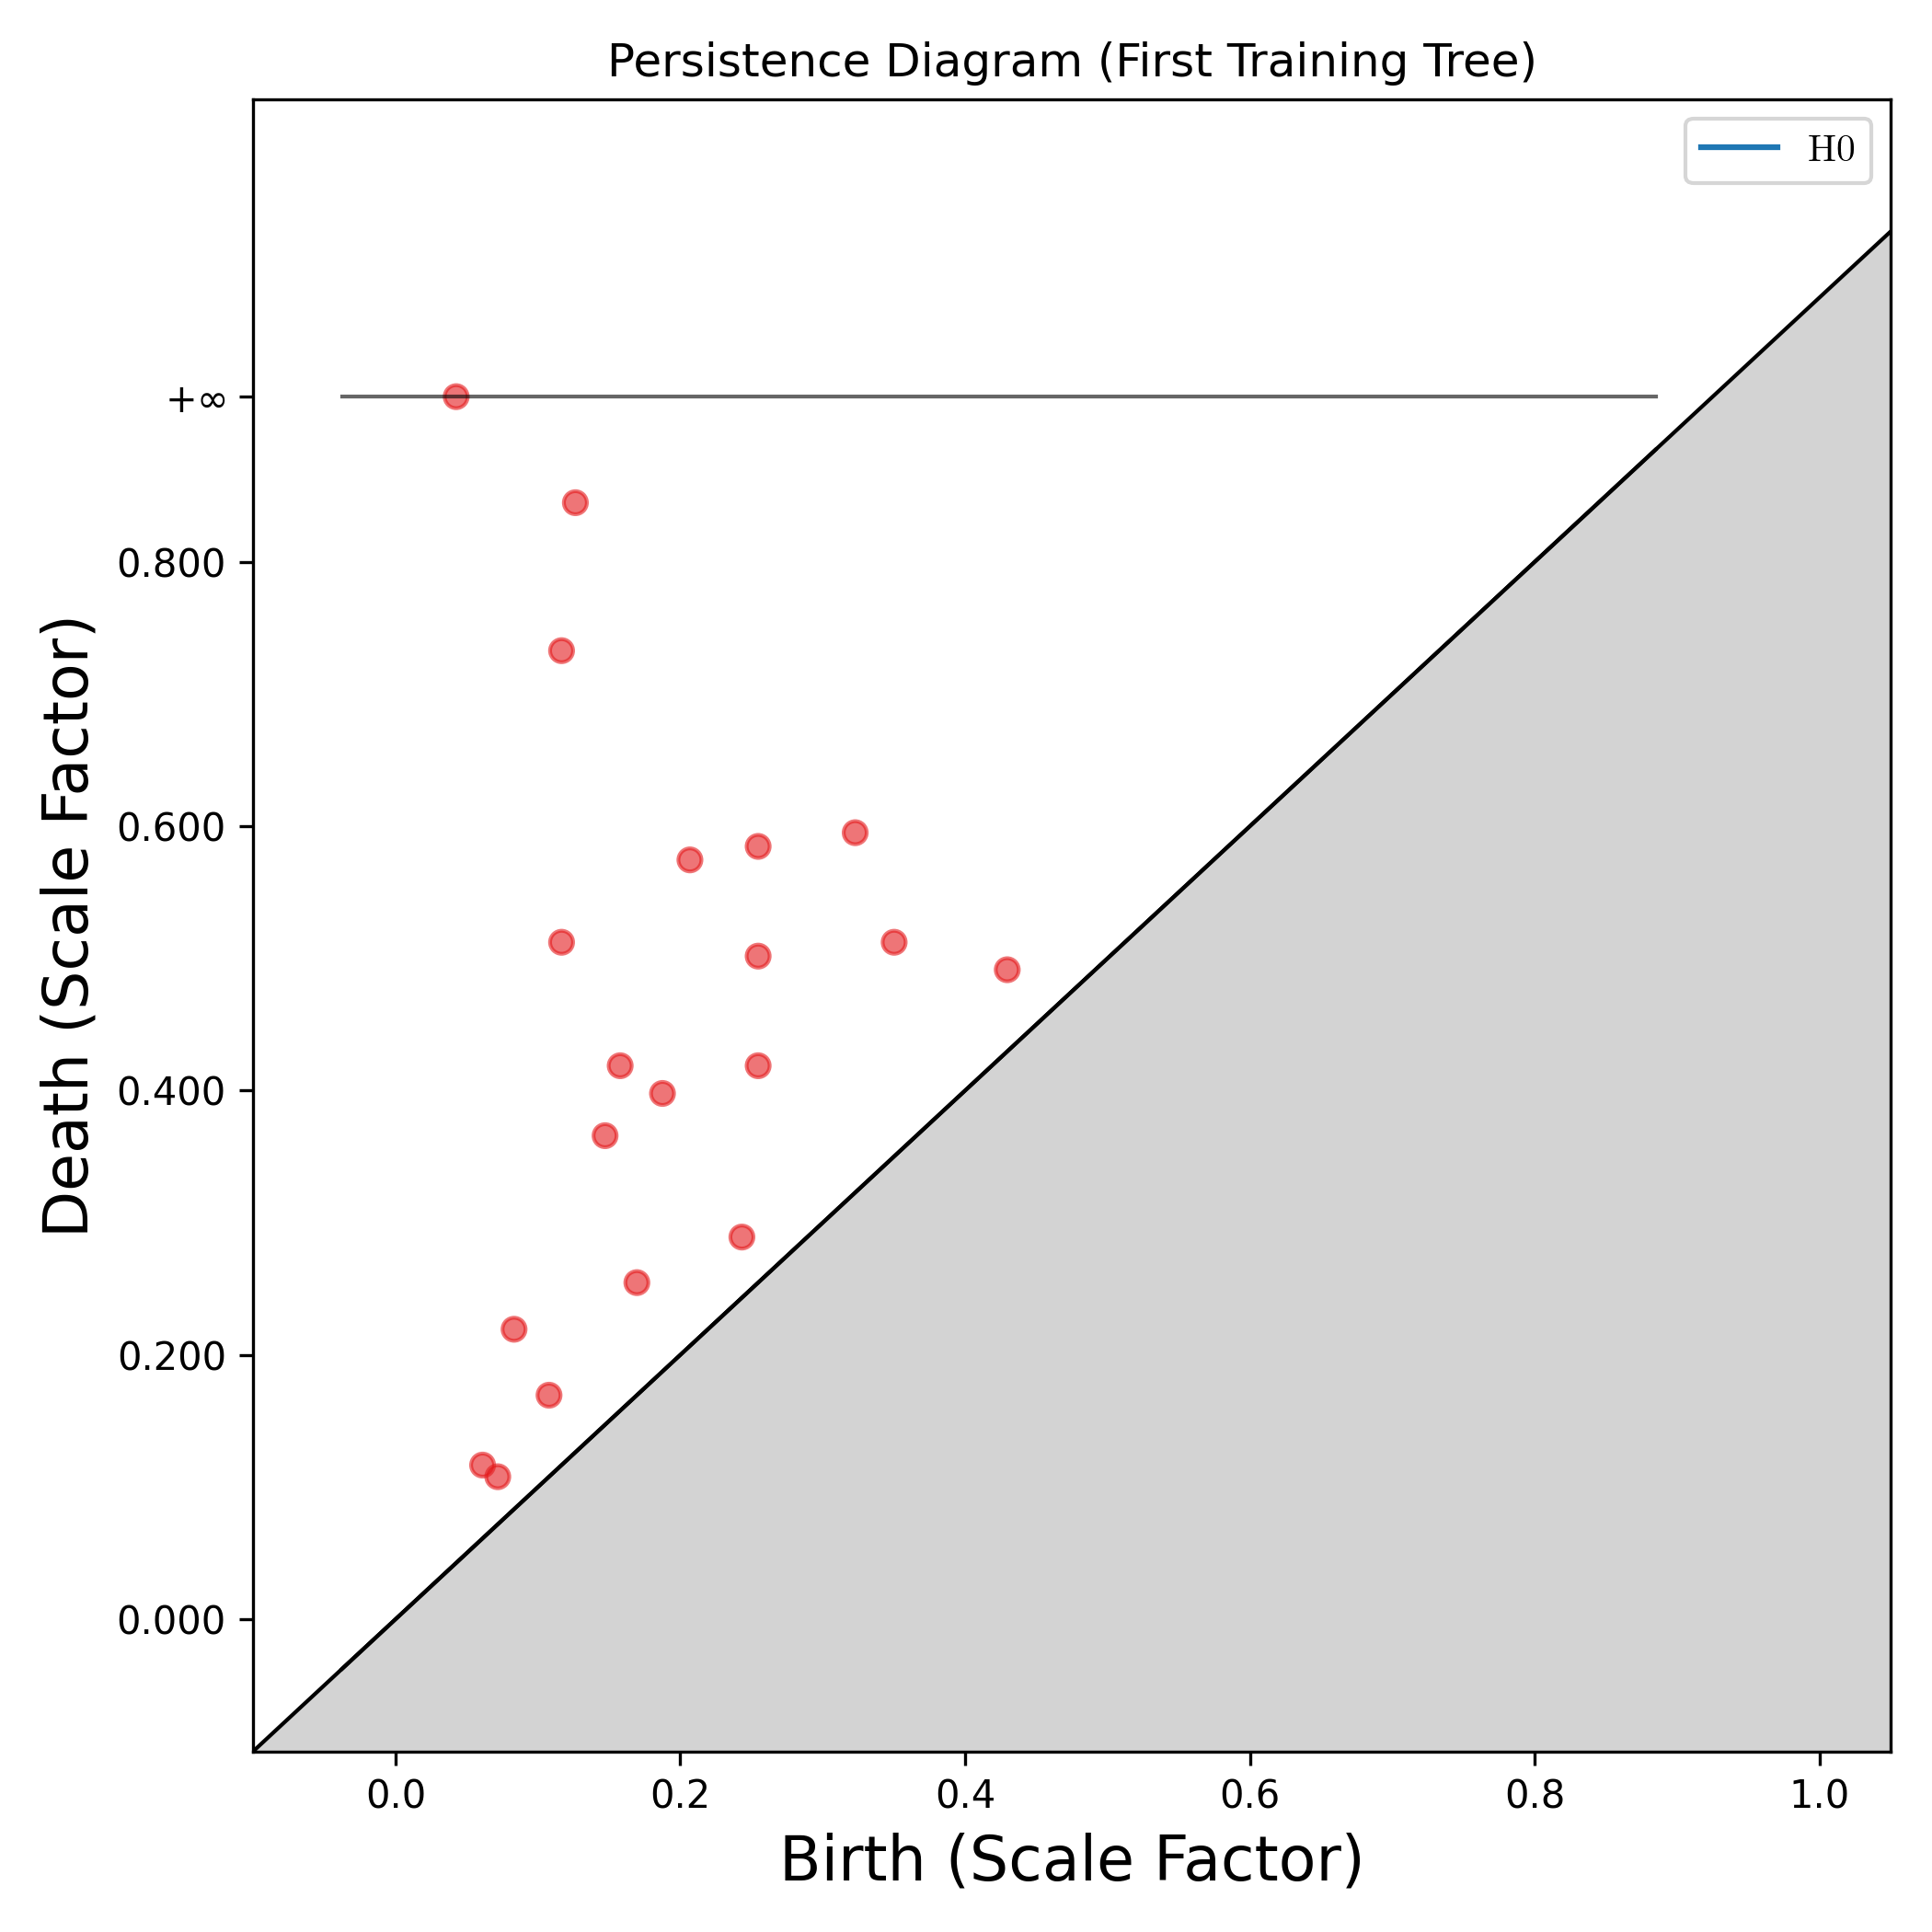
\includegraphics[width=0.5\textwidth]{../input_files/plots/persistence_diagram_1_1748137556.png}
    \caption{\label{fig:persistence_diagram_h0}Persistence diagram (H0) for a sample merger tree, plotting the birth and death times (scale factors) of connected components. The absence of Topological Data Analysis in this study meant that features extracted from such diagrams could not be used to inform the GNN or correlate with the assembly bias proxy.}
\end{figure}

\begin{figure}[htbp]
    \centering
    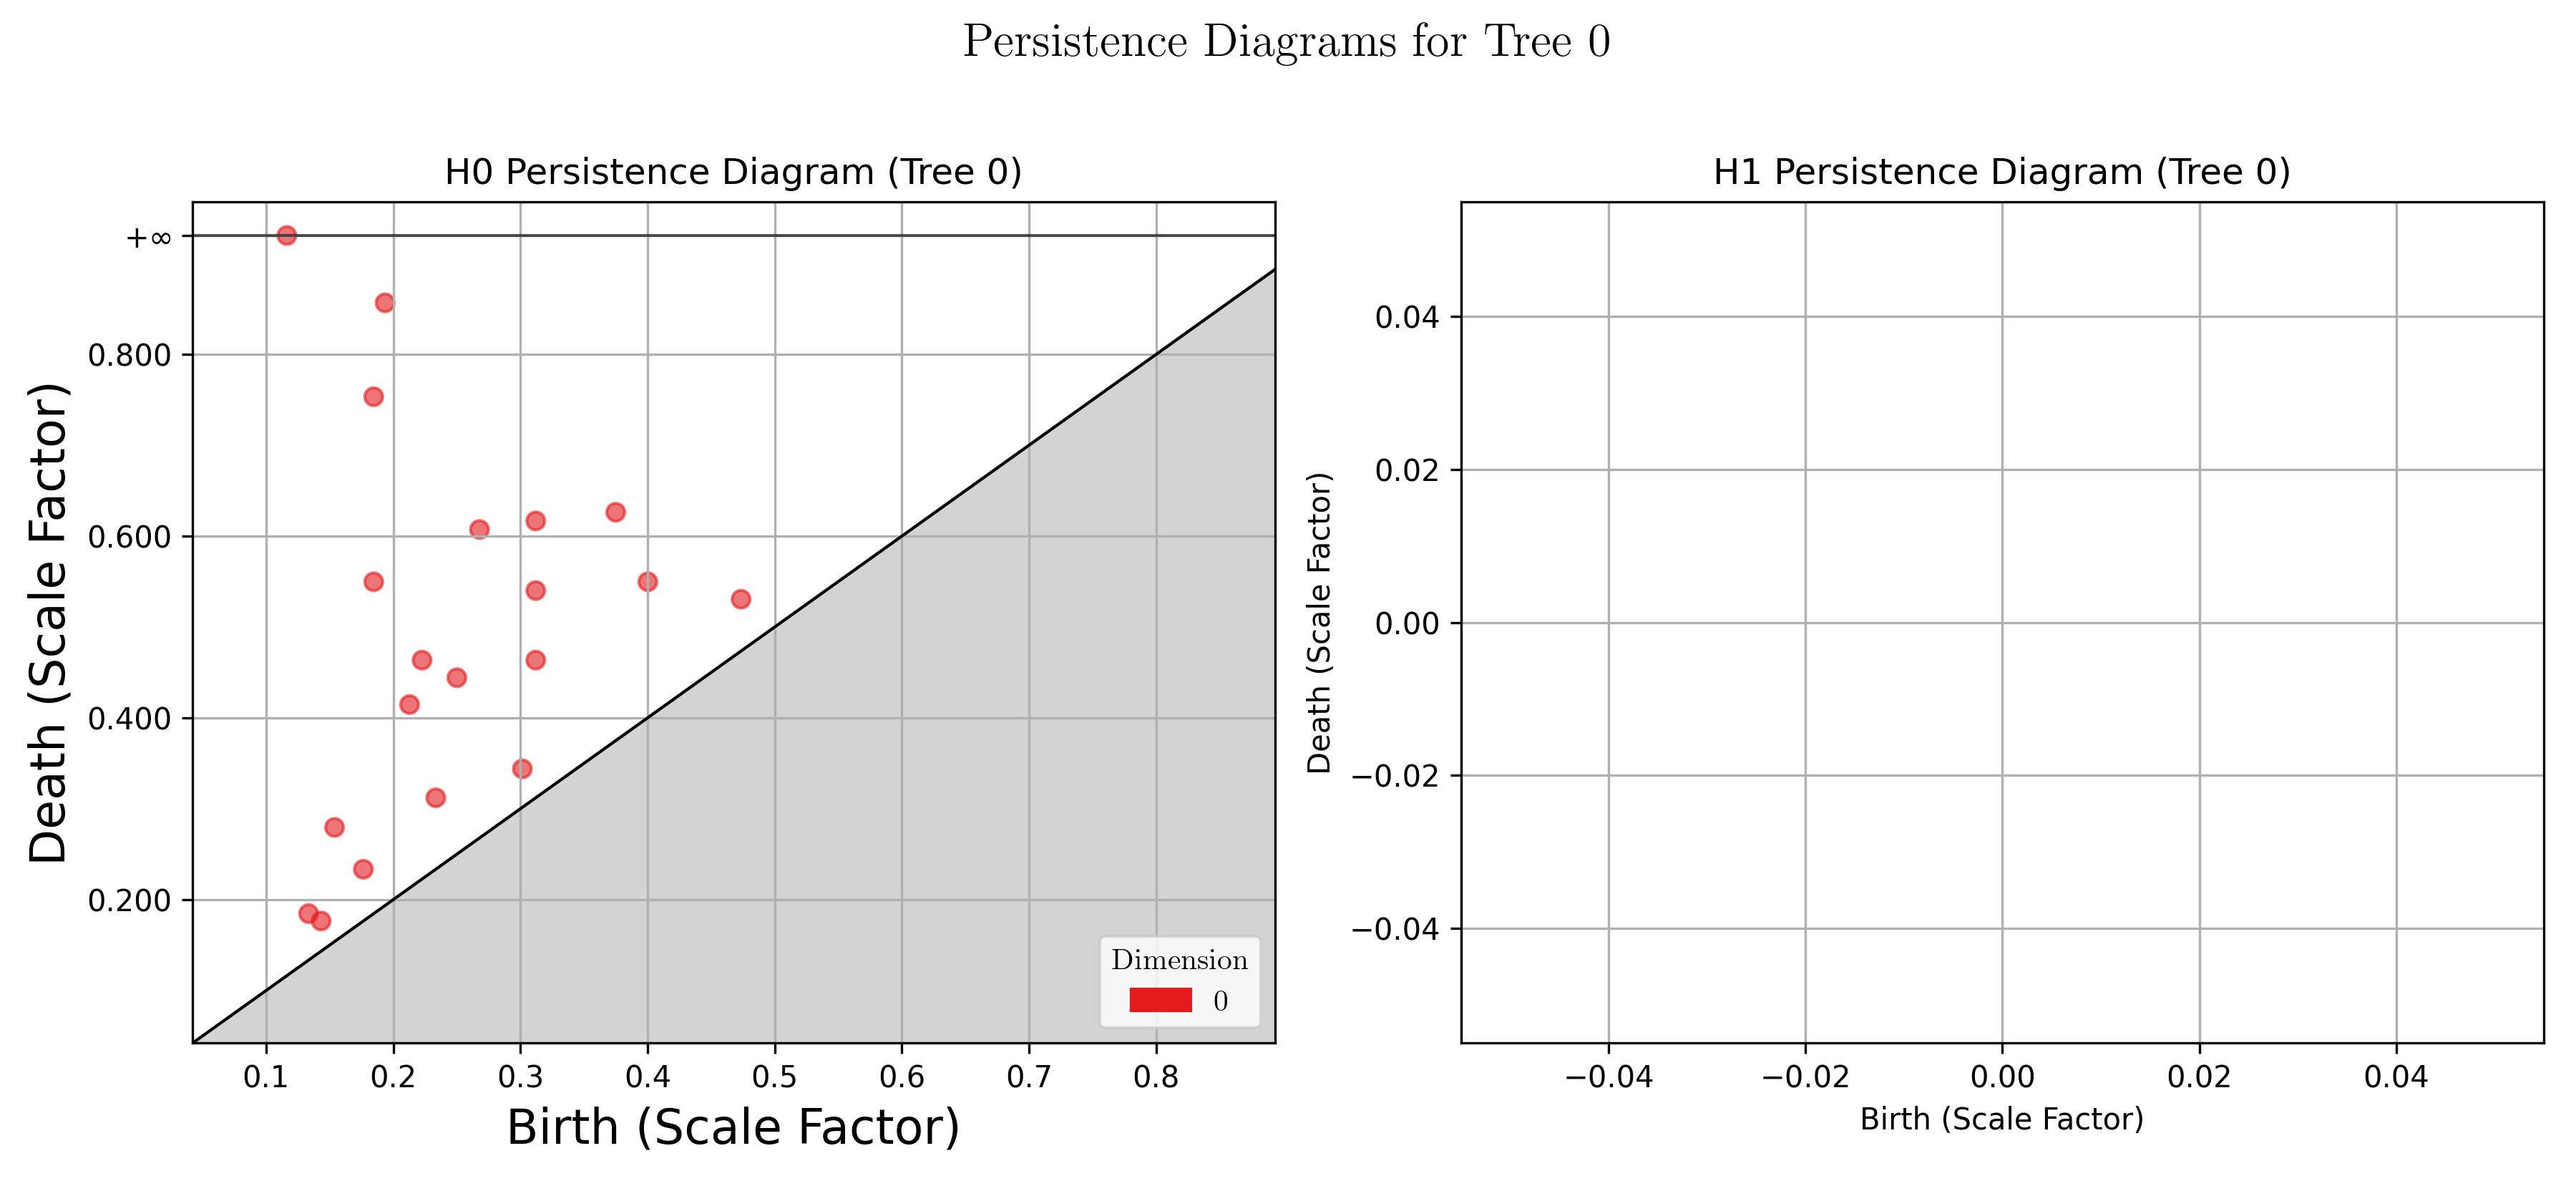
\includegraphics[width=0.5\textwidth]{../input_files/plots/persistence_diagram_tree0_20250524214205.png}
    \caption{\label{fig:persistence_diagram_h0_h1}Persistence diagrams for a sample merger tree, displaying the birth and death scale factors of topological features (connected components in H0 and loops in H1). The H1 diagram is empty, and since Topological Data Analysis was not performed, these diagrams could not inform the GNN.}
\end{figure}

\begin{figure}[htbp]
    \centering
    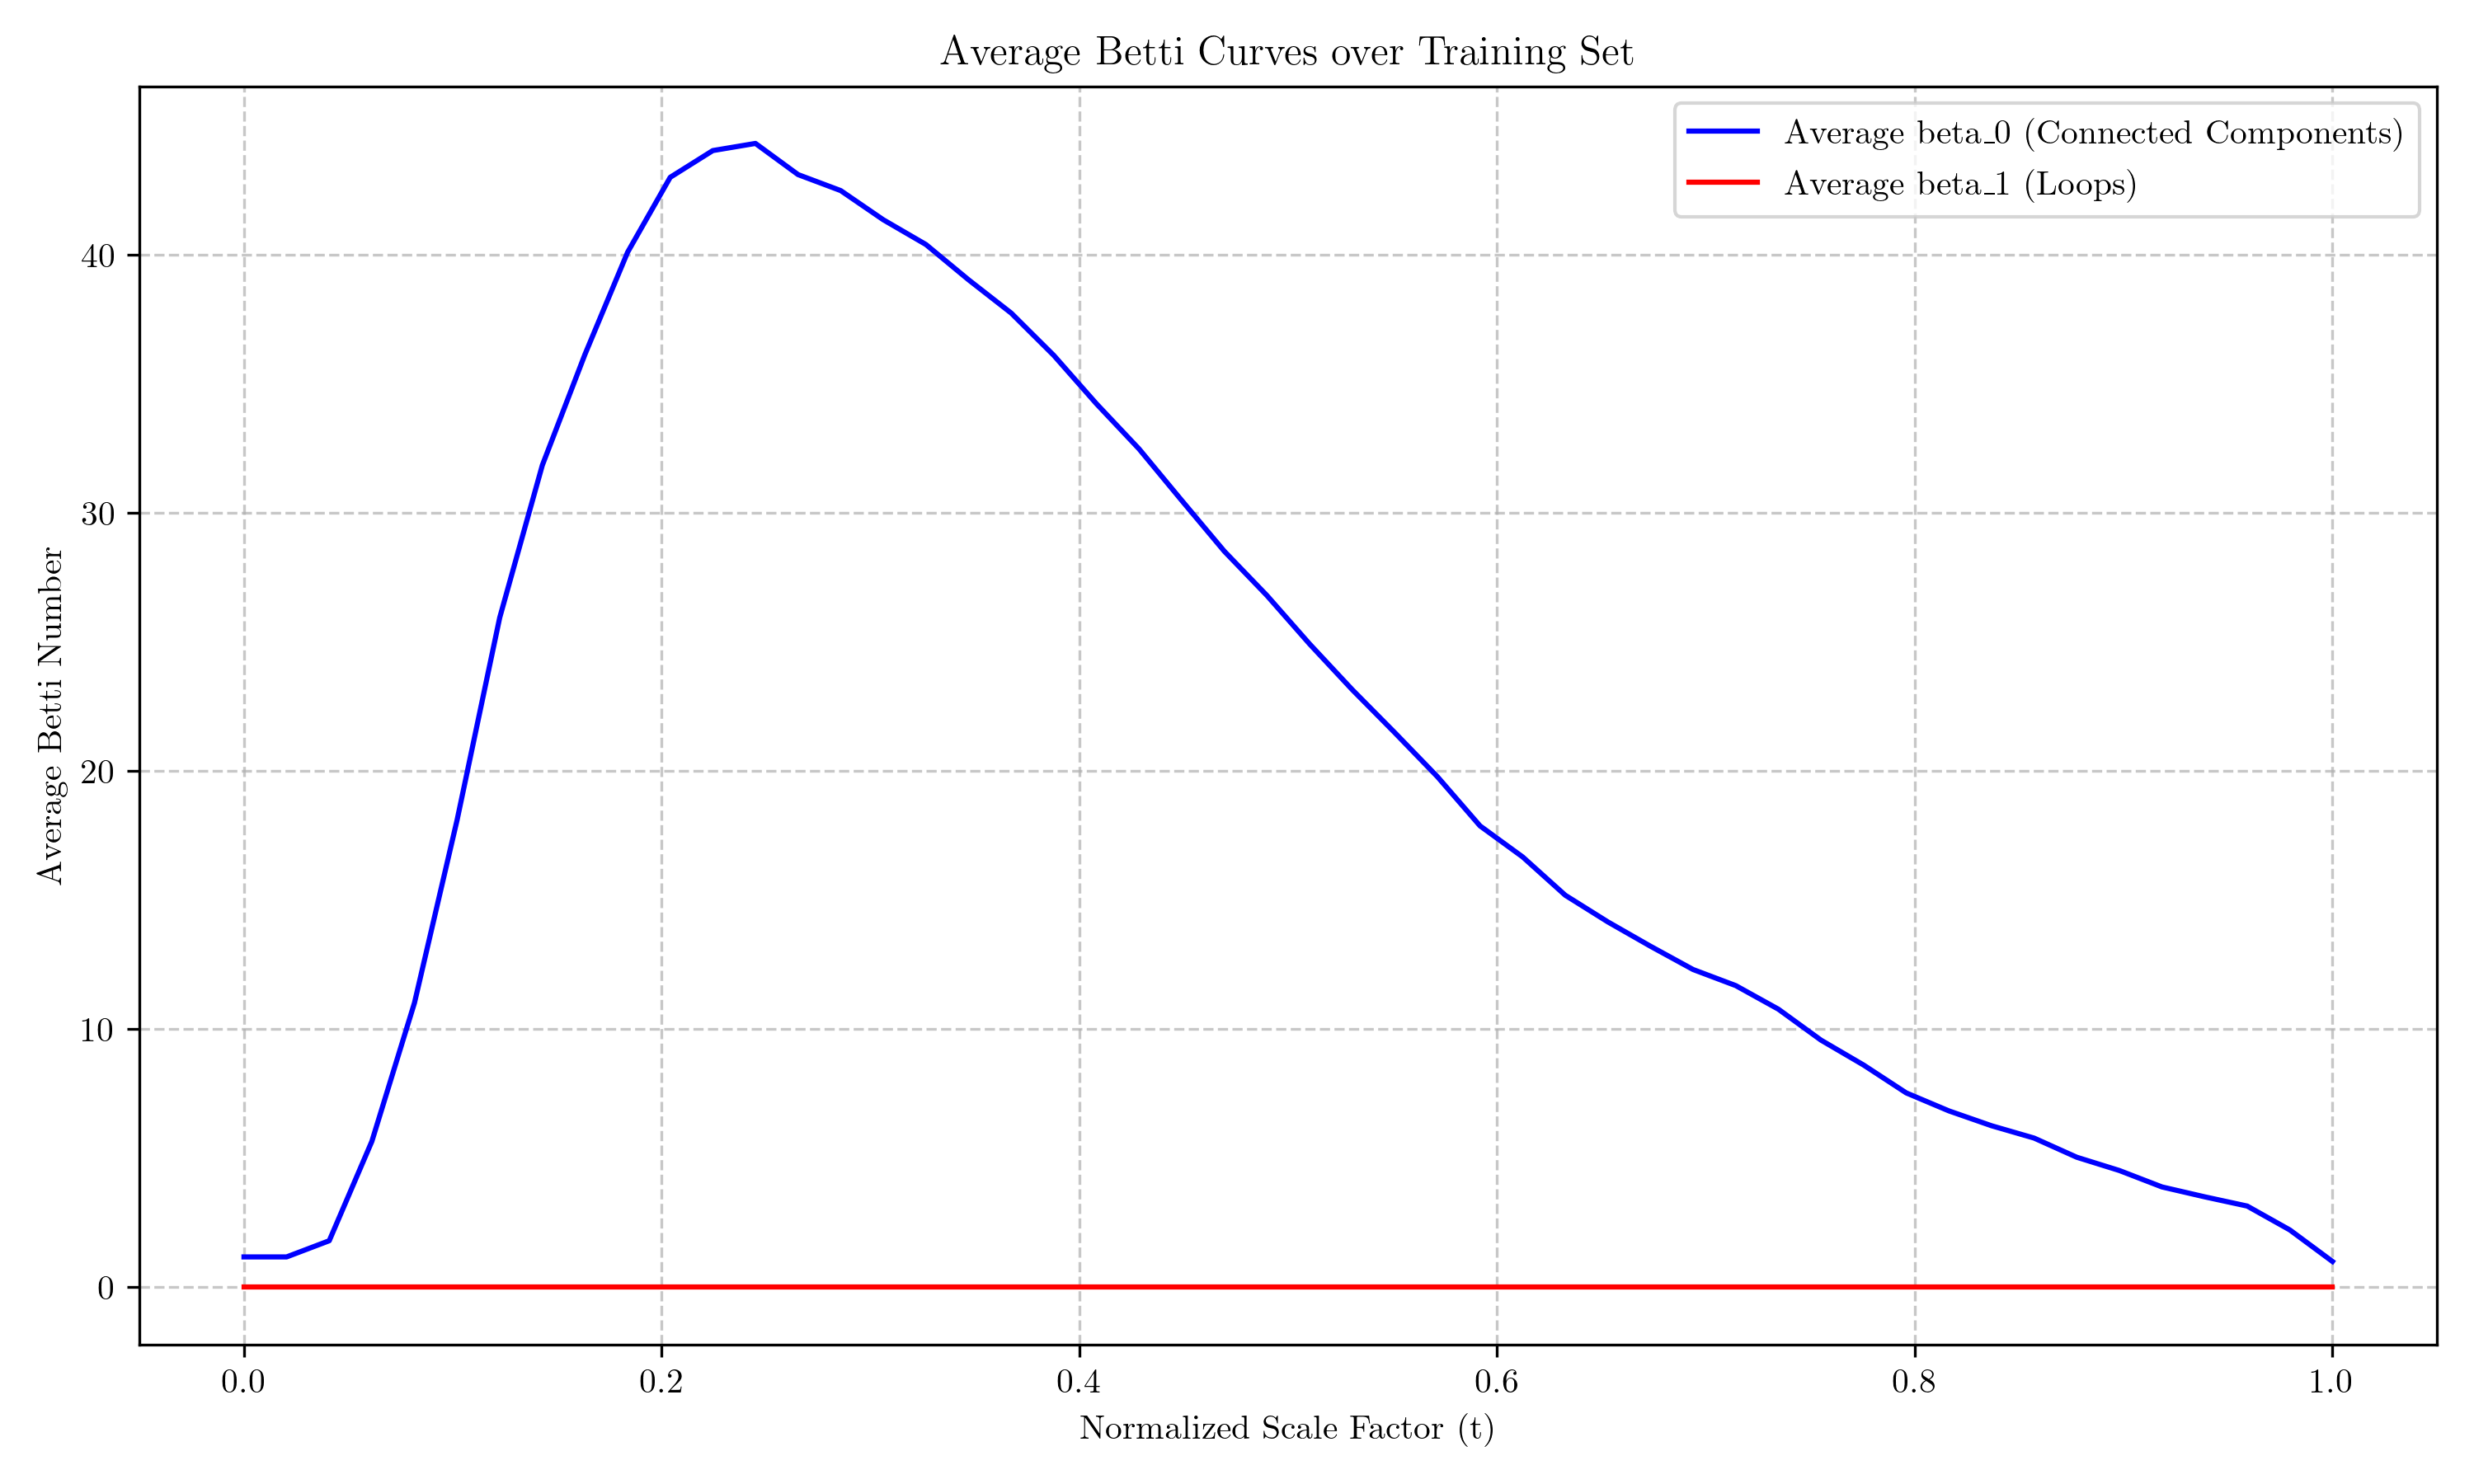
\includegraphics[width=0.5\textwidth]{../input_files/plots/avg_betti_curves_2_1748137556.png}
    \caption{\label{fig:avg_betti_numbers}Average Betti numbers (H0 and H1) as a function of normalized scale factor, averaged over the training set merger trees. The Topological Data Analysis, which would have used these features, was not executed in this study.}
\end{figure}

\subsection{Graph Neural Network (GNN) Model Performance}

A Graph Convolutional Network (GCN) was designed and implemented using PyTorch Geometric to predict the assembly bias proxy from the preprocessed merger tree data.

\subsubsection{GNN architecture and training}
As described in the methods section, the GCNNet architecture included:
\begin{itemize}
    \item A node feature encoder (Linear layer).
    \item An edge feature encoder (Linear layer), if edge features were present.
    \item A configurable number of \texttt{GCNConv} layers with ReLU activation.
    \item A global mean pooling layer to aggregate node embeddings into a graph-level embedding.
    \item A final linear regression layer to output the scalar assembly bias proxy.
\end{itemize}

Hyperparameter tuning was attempted for the number of GCN layers ([1, 2]) and the number of hidden channels ([16, 32]). Other training parameters were fixed:
\begin{itemize}
    \item Learning Rate: 0.0001
    \item Batch Size: 4
    \item Number of Epochs: 50
    \item Optimizer: Adam
    \item Loss Function: Mean Squared Error (MSE)
    \item Weight Decay: 1e-5
\end{itemize}

\subsubsection{Hyperparameter tuning and training instability}
The hyperparameter tuning phase revealed significant issues, particularly with smaller network configurations.
\begin{itemize}
    \item Models with \texttt{hidden\ensuremath{\_}channels: 16} (for both 1 and 2 GCN layers) consistently produced \texttt{NaN} (Not a Number) losses during training and validation. This indicates severe training instability, possibly due to vanishing/exploding gradients, issues with the very small batch sizes relative to model complexity (even if small), or numerical precision problems exacerbated by the extremely limited data. Gradient clipping was implemented, but it was not sufficient to prevent NaNs in these cases.
\end{itemize}

The configurations with \texttt{hidden\ensuremath{\_}channels: 32} were trainable:
\begin{itemize}
    \item \textbf{1 GCN layer, 32 hidden channels:} Achieved the best validation MSE of \textbf{104.7496}.
    \item \textbf{2 GCN layers, 32 hidden channels:} Achieved a validation MSE of \textbf{105.6353}.
\end{itemize}

While both training and validation losses show a decreasing trend over the 50 epochs, the final MSE values are extraordinarily high. For context, the variance of the target variable (assembly bias proxy) in the dataset is approximately 0.734. An MSE exceeding 100 is orders of magnitude larger, suggesting the model has learned very little, if anything, about the underlying relationship between the input features and the target.

\begin{figure}[htbp]
    \centering
    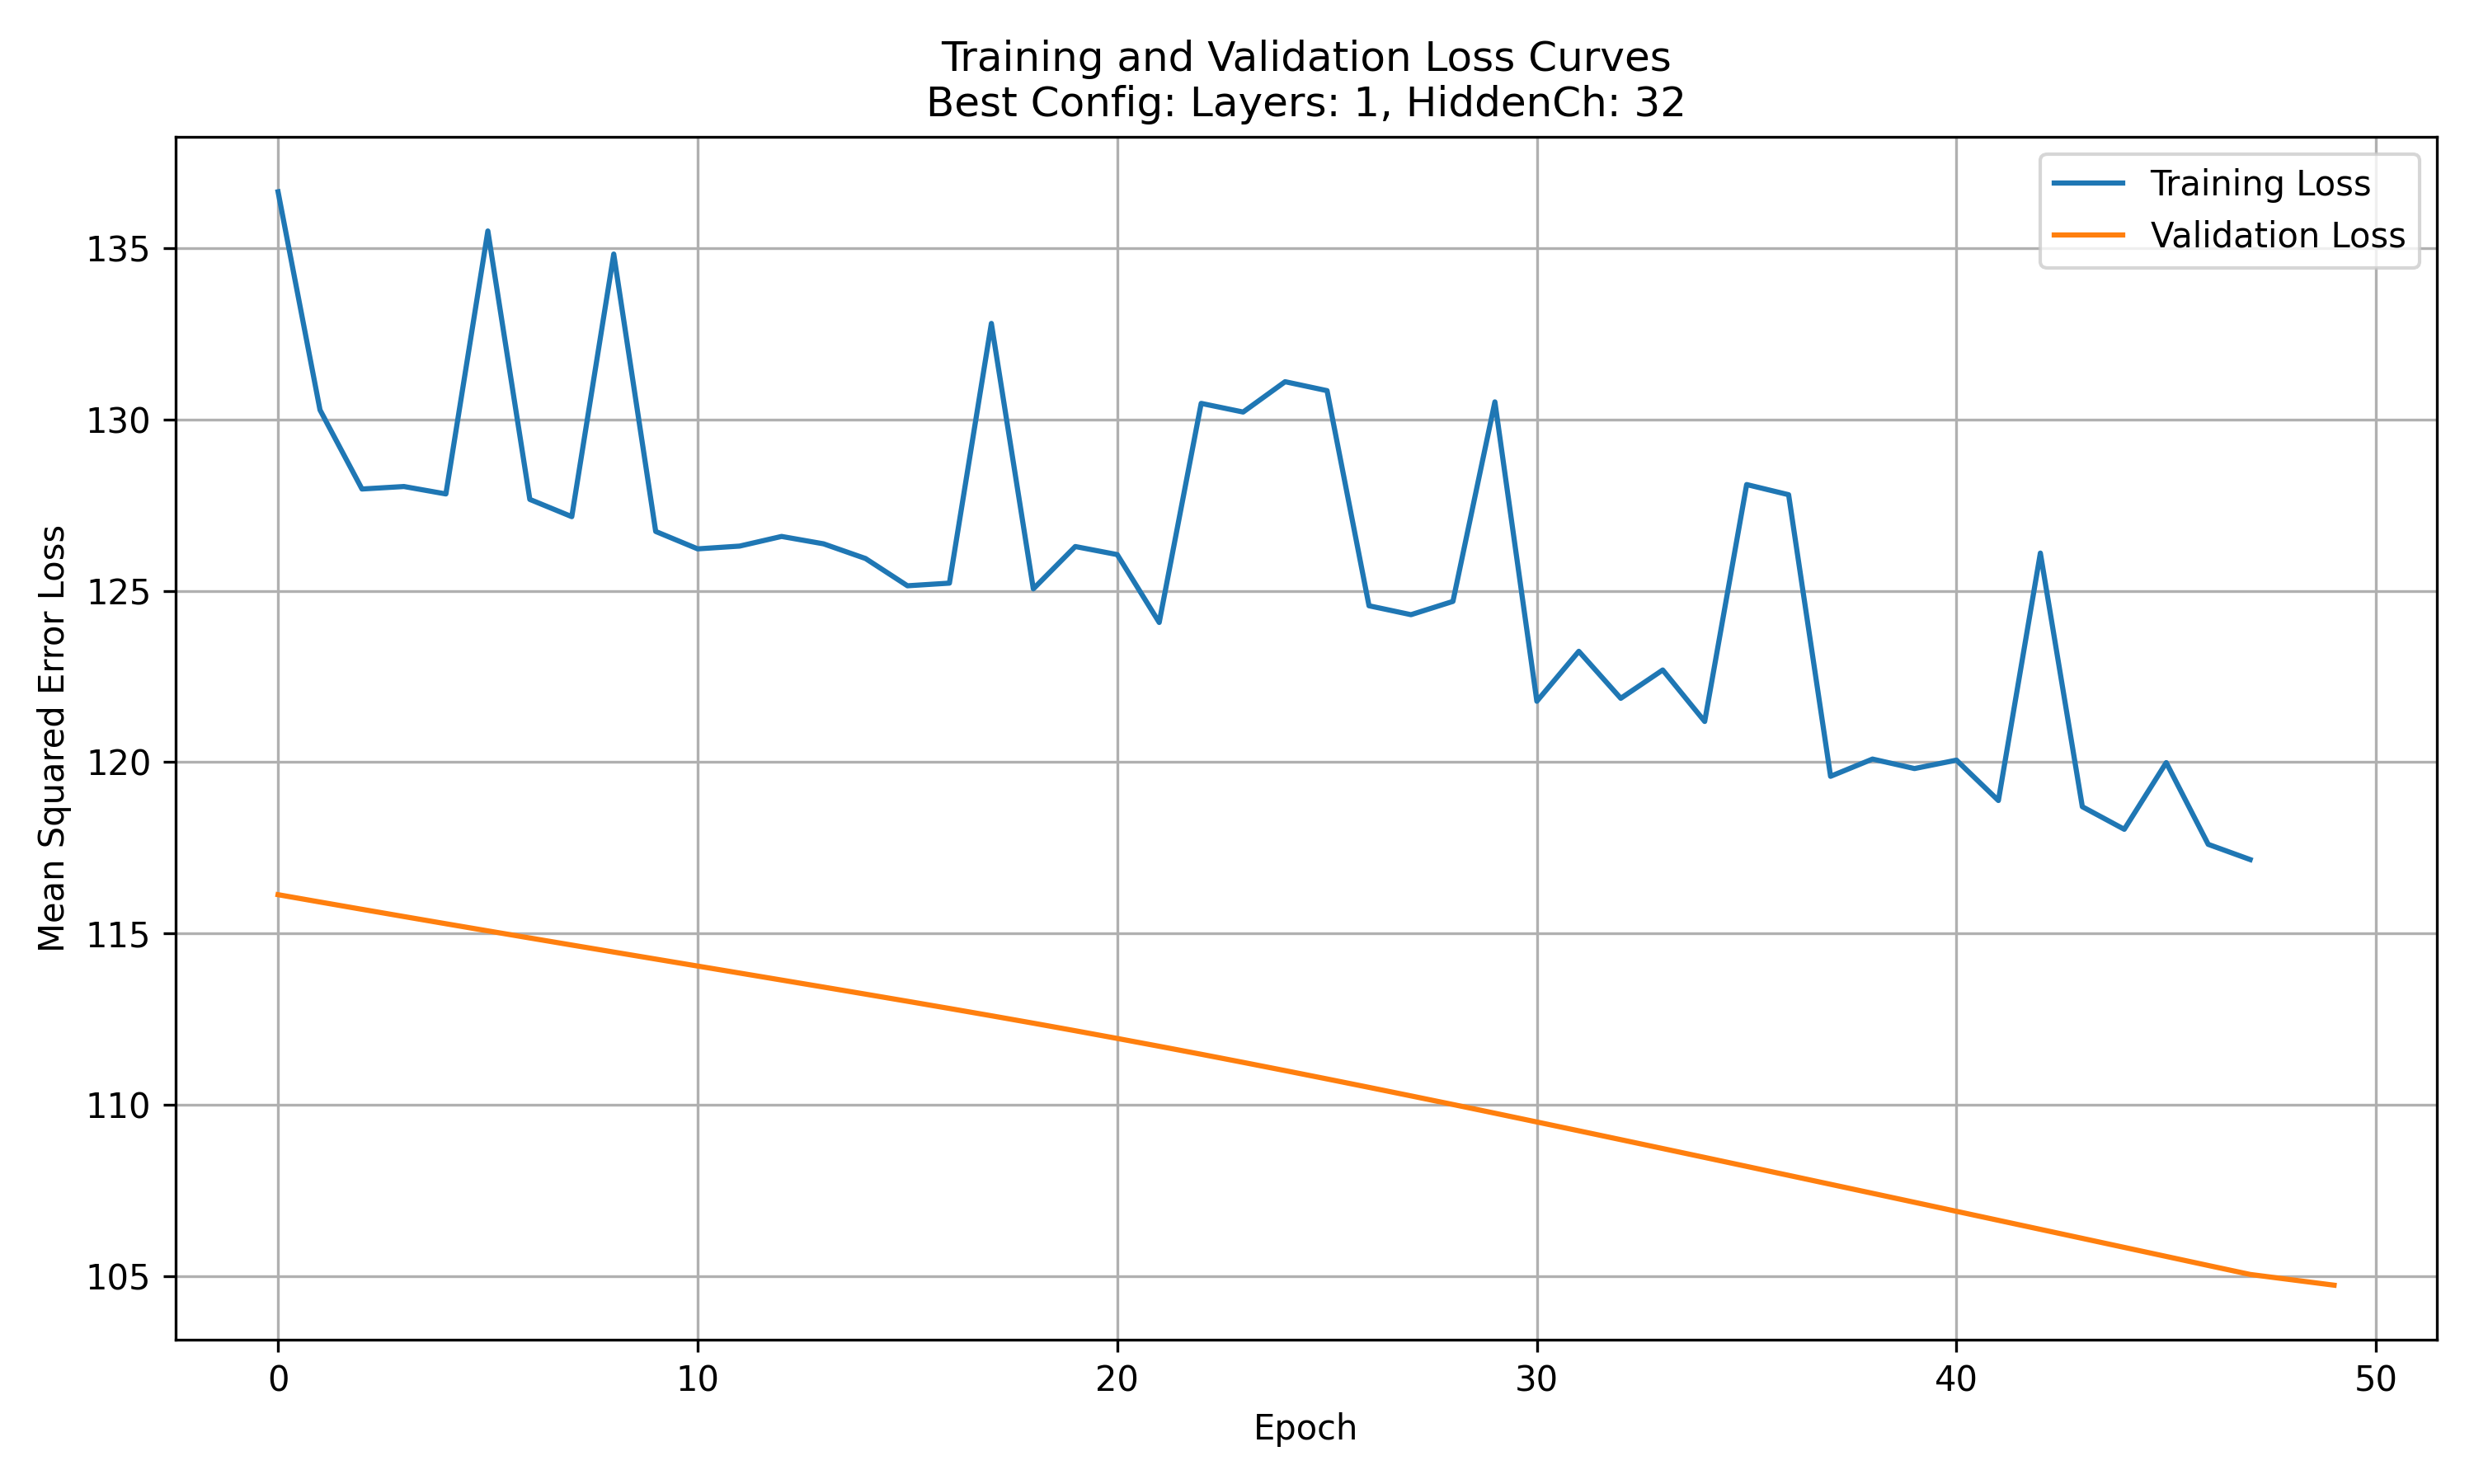
\includegraphics[width=0.5\textwidth]{../input_files/plots/training_validation_loss_curves_plot_1_1748137938.png}
    \caption{\label{fig:training_validation_loss}Training and validation loss curves for the GNN model with 1 GCN layer and 32 hidden channels. The high MSE values indicate the model did not learn the relationship between merger tree features and the assembly bias proxy, likely due to the limited dataset size.}
\end{figure}

\subsubsection{Test set evaluation}
The GNN model with the best hyperparameters (1 GCN layer, 32 hidden channels, validation MSE $\approx$ 104.75) was evaluated on the test set, which comprised only 5 samples. The performance metrics were:
\begin{itemize}
    \item \textbf{Mean Squared Error (MSE): 107.6264}
    \item \textbf{R-squared ($R^2$): -480.5708}
\end{itemize}

\textbf{Interpretation of Test Metrics:}
\begin{itemize}
    \item \textbf{MSE:} An MSE of 107.63 on the test set is consistent with the high validation MSE. It confirms that the model's poor performance generalizes to unseen data (albeit a tiny amount). This value is drastically higher than the variance of the target variable (0.734), indicating that the model's predictions are, on average, very far from the true values.
    \item \textbf{R-squared ($R^2$):} A negative $R^2$ value, such as the \textbf{-480.5708} observed here, signifies an exceptionally poor fit. It means that the model's predictions are substantially worse than simply predicting the mean of the assembly bias proxy for all test samples. The sum of squared residuals (errors) from the model is vastly larger than the total sum of squares (variance of the data).
\end{itemize}

\begin{figure}[htbp]
    \centering
    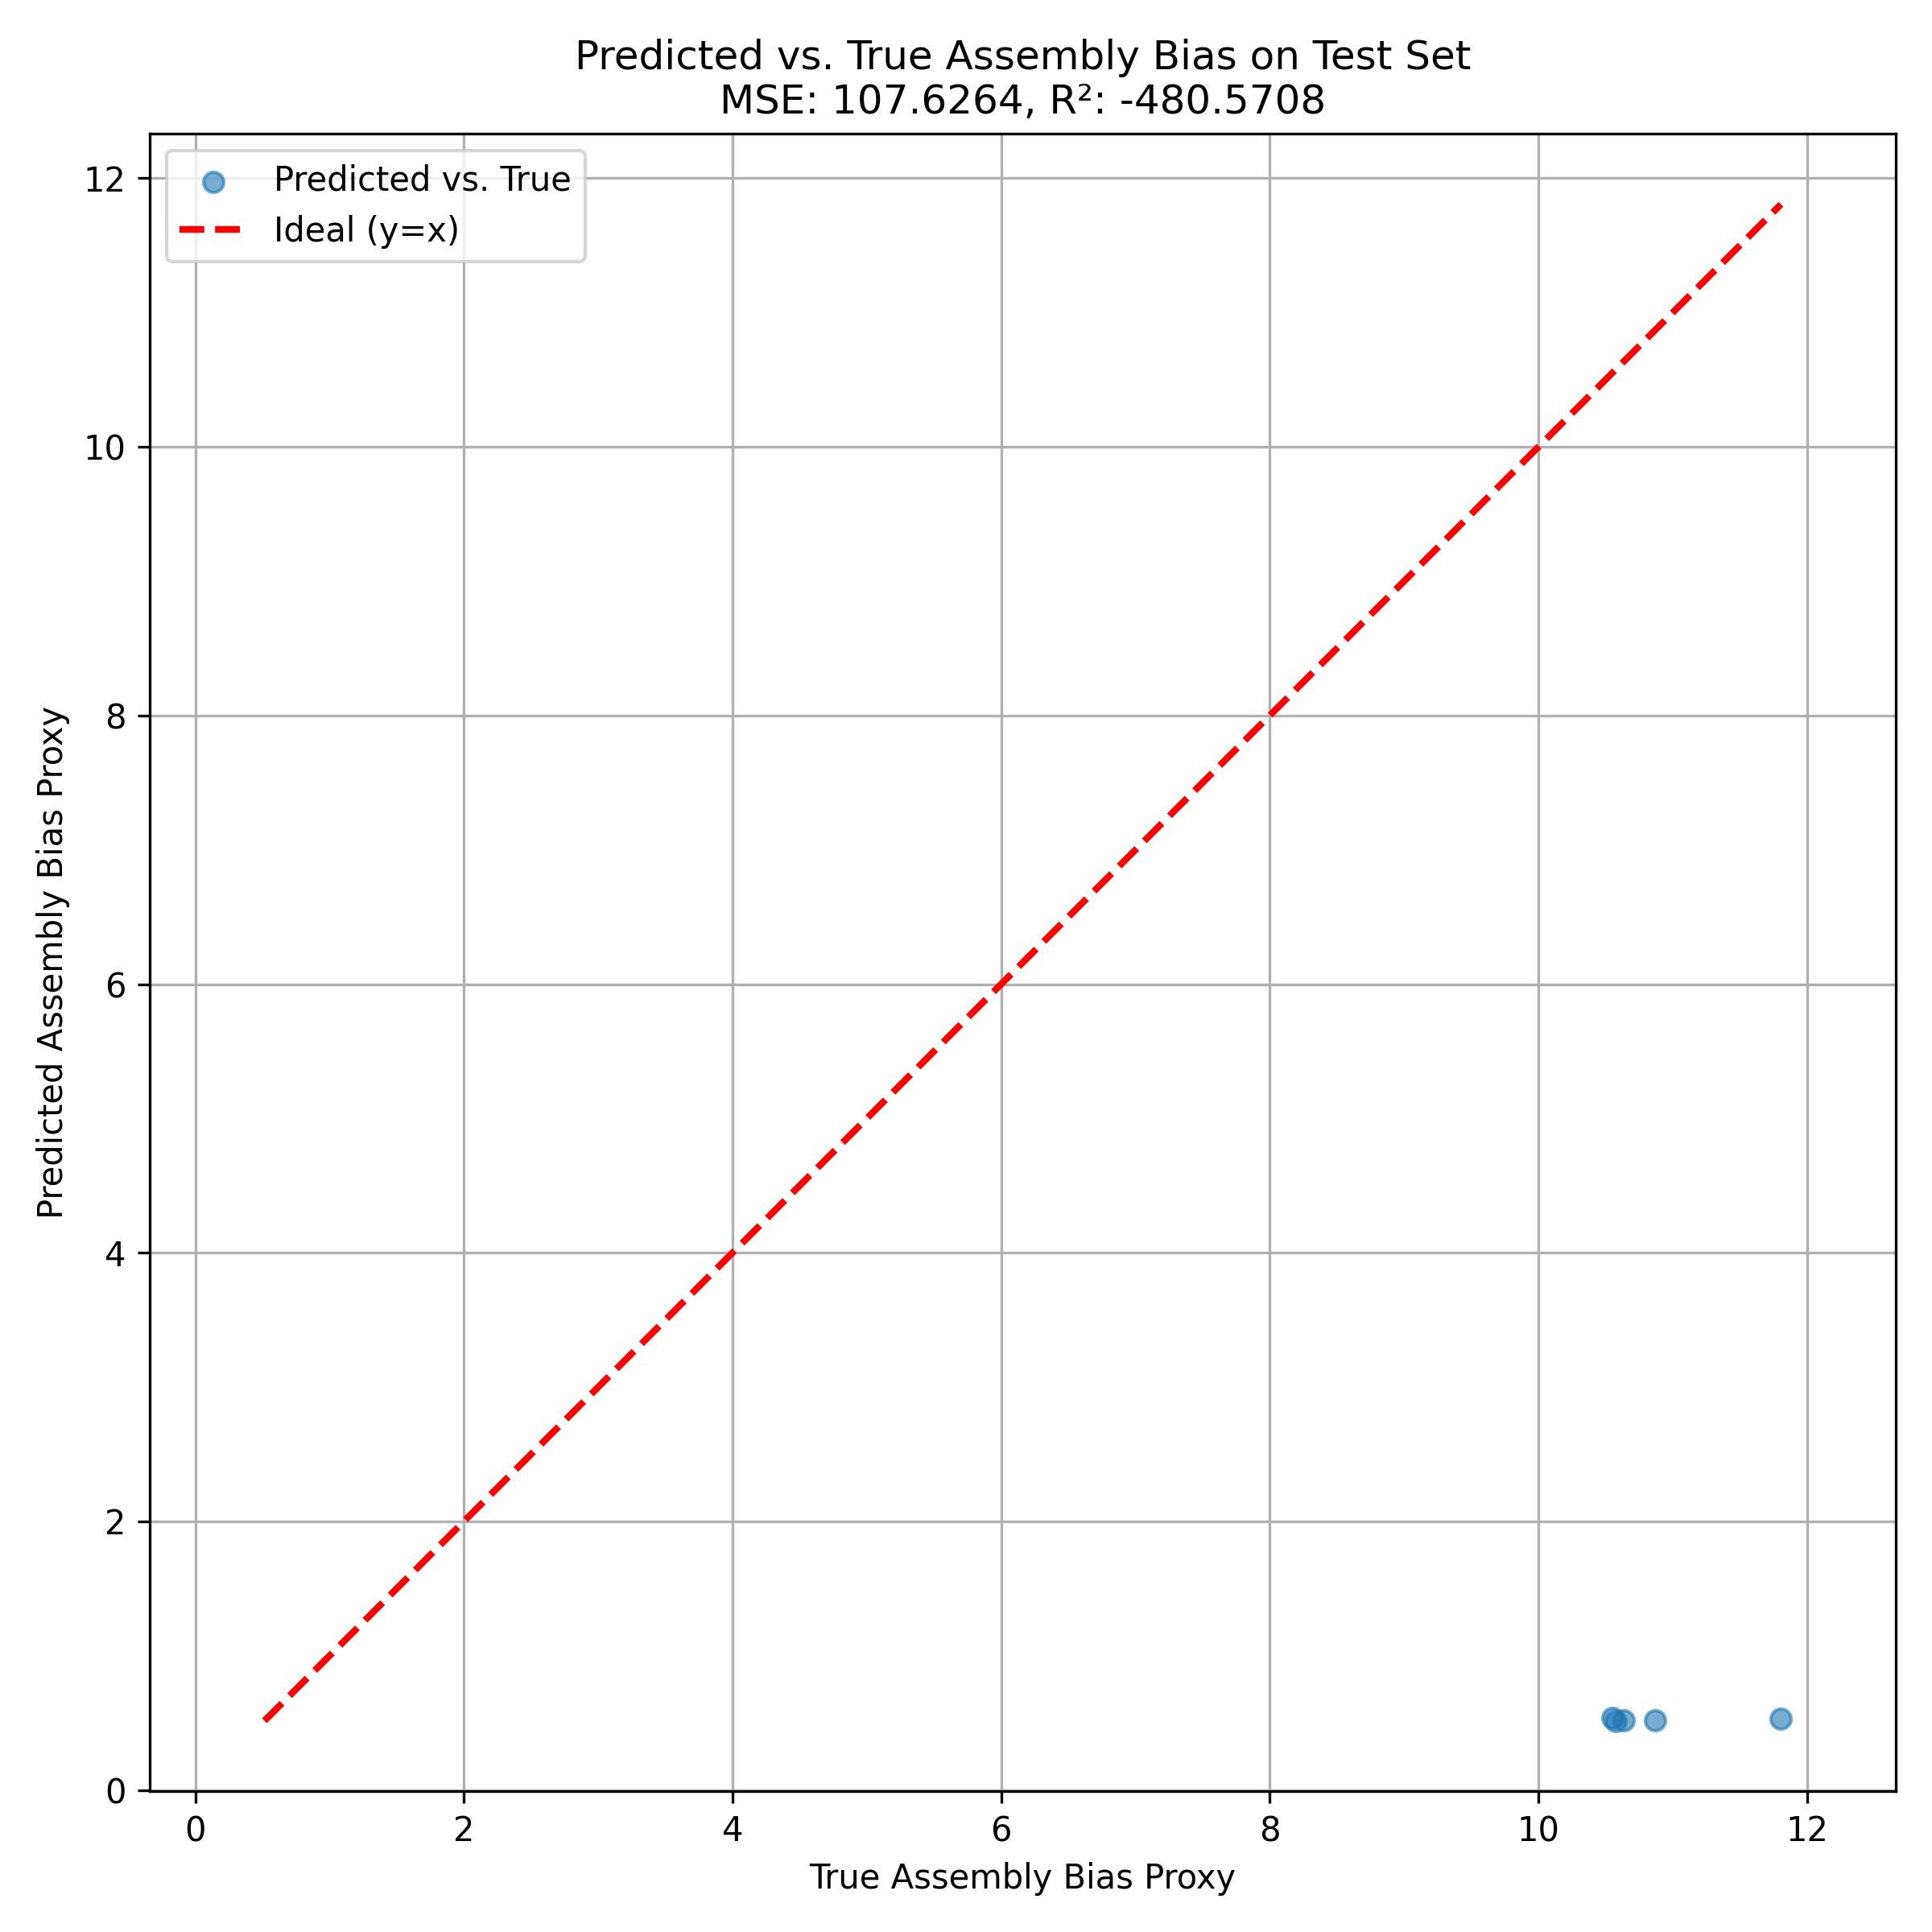
\includegraphics[width=0.5\textwidth]{../input_files/plots/predicted_vs_true_bias_plot_2_1748137938.png}
    \caption{\label{fig:predicted_vs_true}Scatter plot of the GNN's predicted assembly bias proxy values against the true values for the test set. The points are scattered far from the ideal y=x line (red dashed line), indicating a poor predictive performance, as reflected by the high Mean Squared Error (MSE) and the large negative R-squared ($R^2$) value.}
\end{figure}

\subsection{Summary}

The primary outcome of this investigation is that the GNN model, under the severe constraint of an extremely limited dataset (N=25), failed to demonstrate any meaningful predictive capability for the assembly bias proxy based on merger tree morphology. The quantitative metrics (high MSE, large negative $R^2$) unequivocally point to a model that has not learned the underlying patterns in the data. The inability to reliably compute the assembly bias proxy for the majority of merger trees severely hampered the analysis and highlights the critical importance of data quality and sufficient sample size for training complex machine learning models. The planned Topological Data Analysis component could not be implemented due to the data limitations, precluding the exploration of potential synergies between TDA and GNNs.

\begin{figure}[htbp]
    \centering
    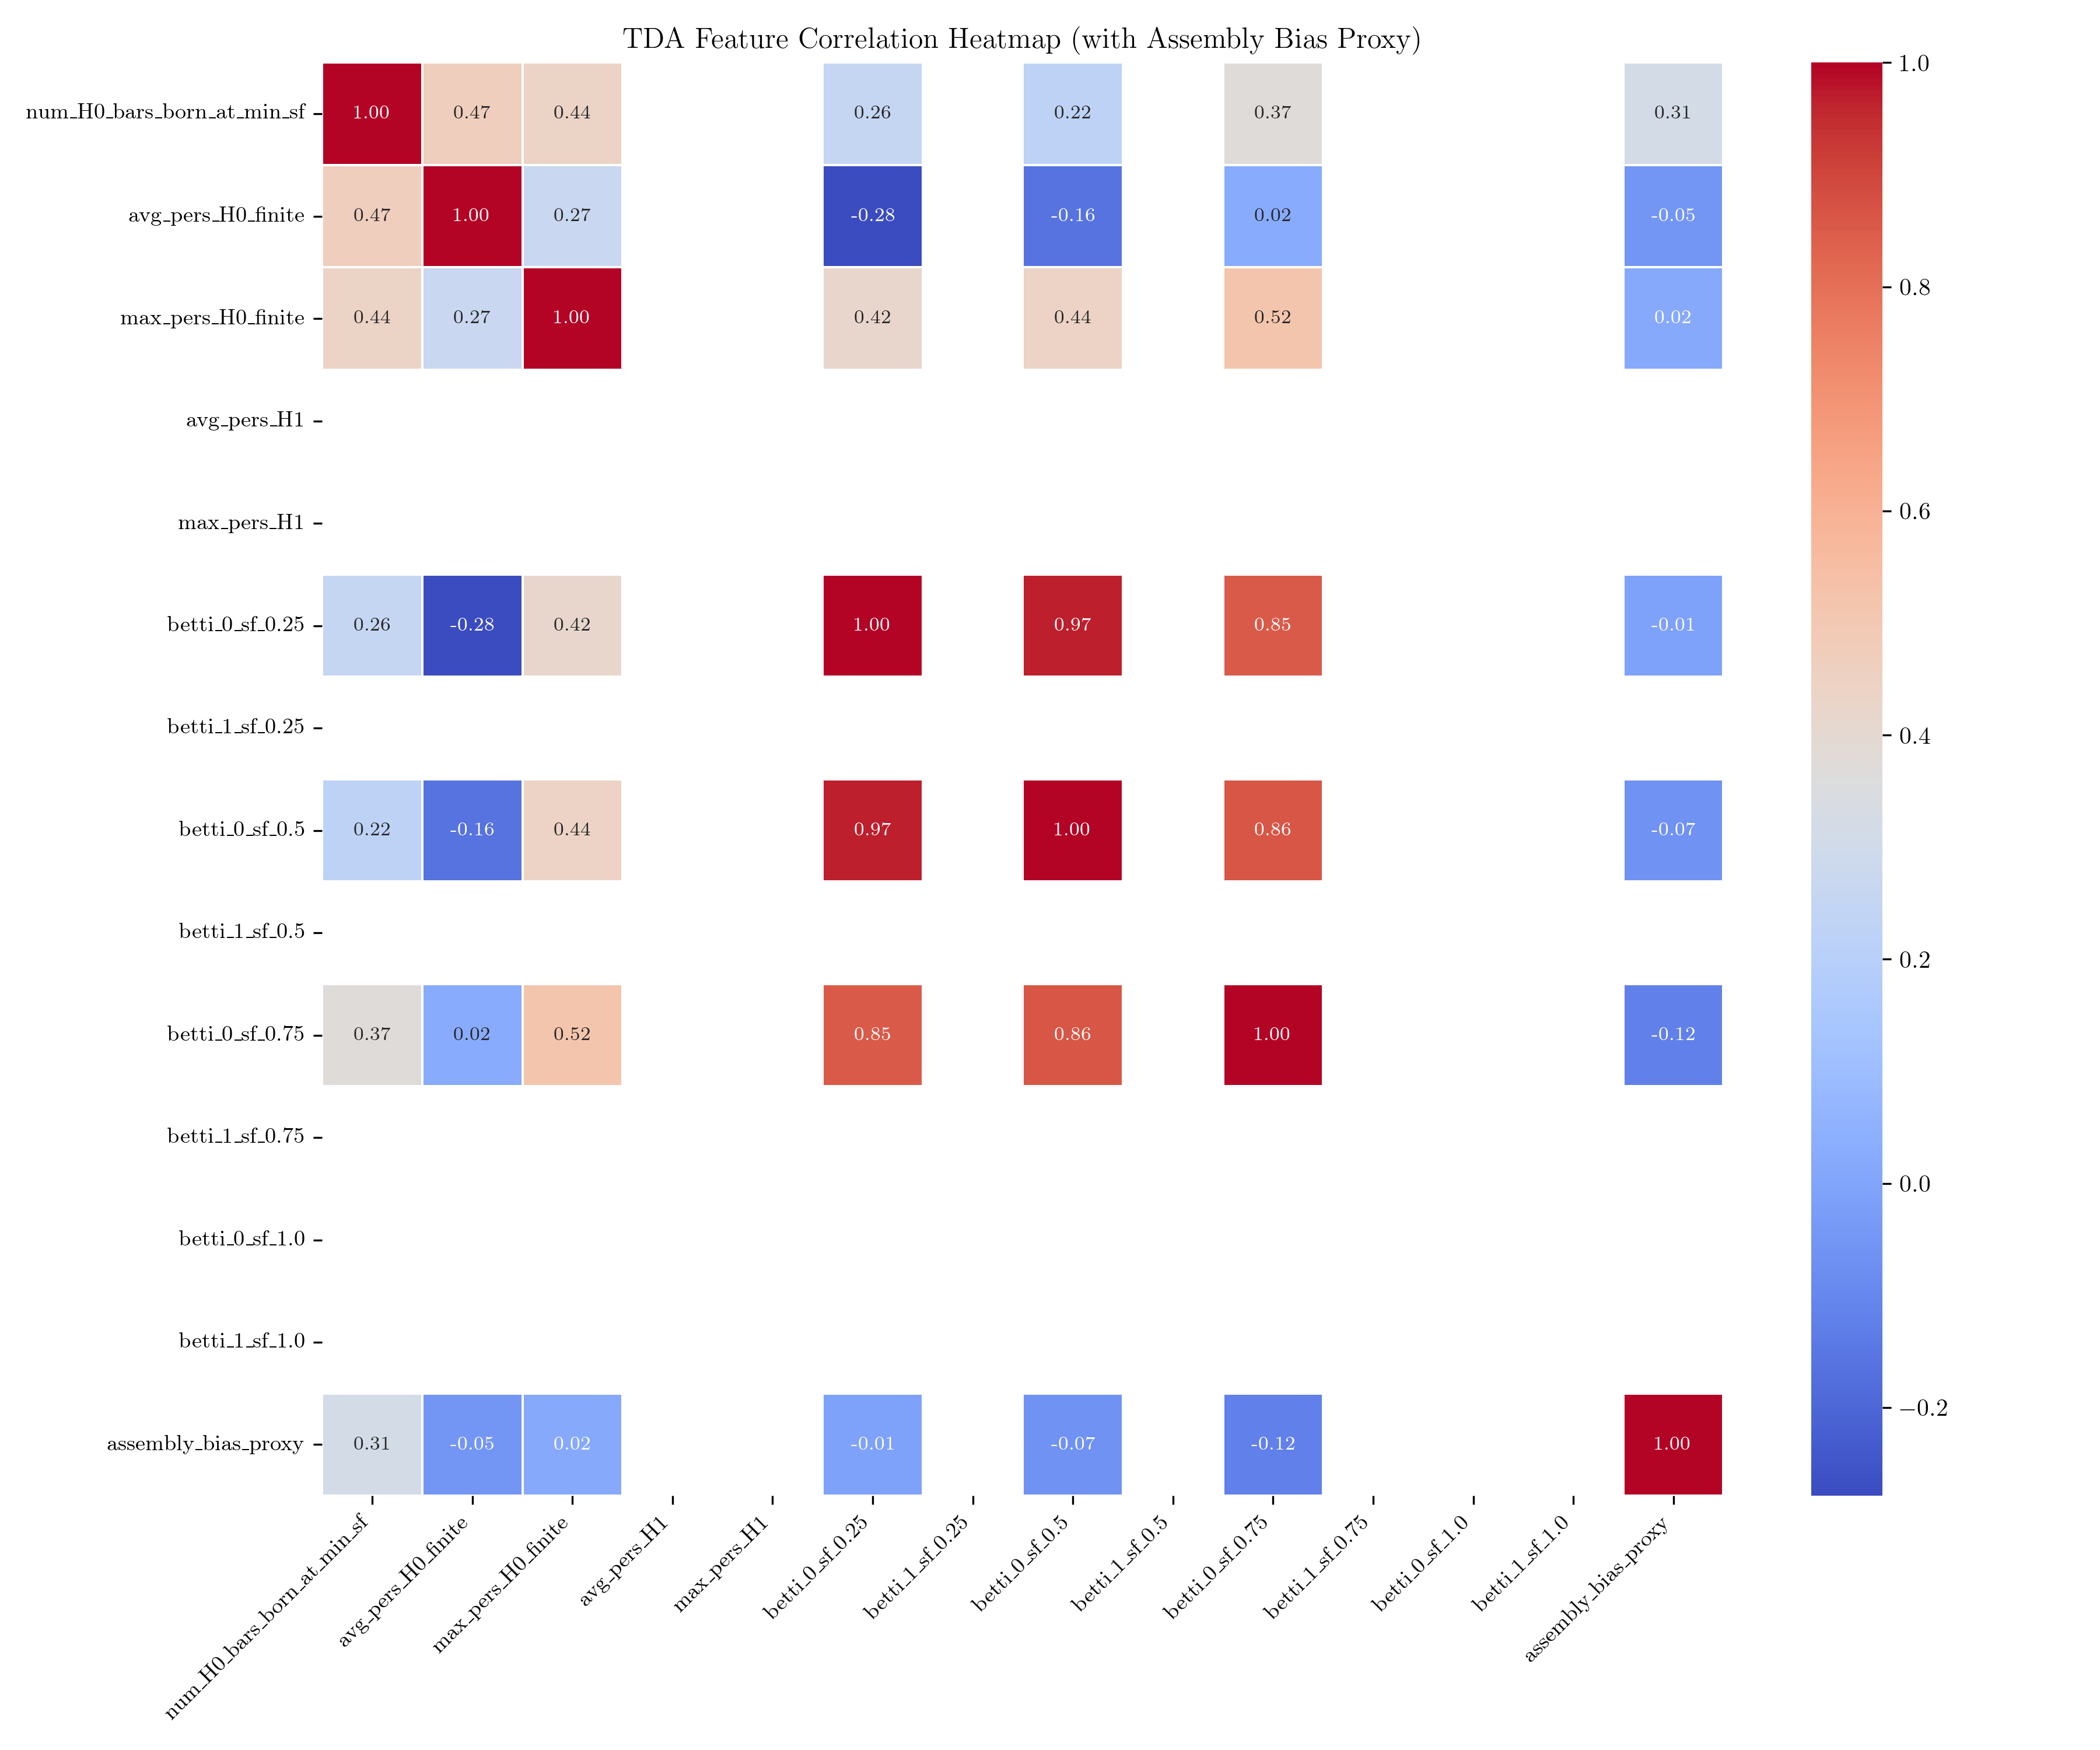
\includegraphics[width=0.5\textwidth]{../input_files/plots/tda_feature_correlation_heatmap_3_1748137556.png}
    \caption{\label{fig:tda_correlation}Correlation heatmap between topological features derived from merger trees and the assembly bias proxy. The lack of strong correlations may explain the limited success of the GNN in predicting the assembly bias proxy.}
\end{figure}

\end{document}
                